\chapter{Stakeholderanalyse}

Für die STH App sind Stakeholder aus verschiedenen Bereichen vorhanden.
Die Applikation erstrebt einen großen Einfluss auf die Sportindustrie und das speziell auf den Prozess des Anwerbens von neuen Fußballspielern durch Vereine in unterschiedlichen Größen.

Deshalb ist eine Stakeholderanalyse besonders wichtig, um die verschiedenen Gruppen an Interessenten zu identifizieren und zufriedenstellen zu können.
Für die Analyse werden folgende Gruppen an Stakeholdern betrachtet: Interne-, Externe-, Community- und Technische Stakeholder.

\section{Vorgehen Stakeholderanalyse}

Die Stakeholderanalyse wurde mit einem konkreten Vorgehen erstellt.
Zuerst wurde erneut die Größe und Auswirkung der Applikation betrachtet.
Dabei ist es auch wichtig, die Zielsysteme nicht außer Acht zu lassen, um konkrete Benutzergruppen definieren zu können.


\section{Grafische Darstellung Stakeholderanalyse}

In der folgenden Abbildung sind die Stakeholdergruppen und deren Abhängigkeiten aufgezeichnet.

\begin{figure}
	\caption[Stakeholderanalyse]{Stakeholderanalyse}
	\centering
	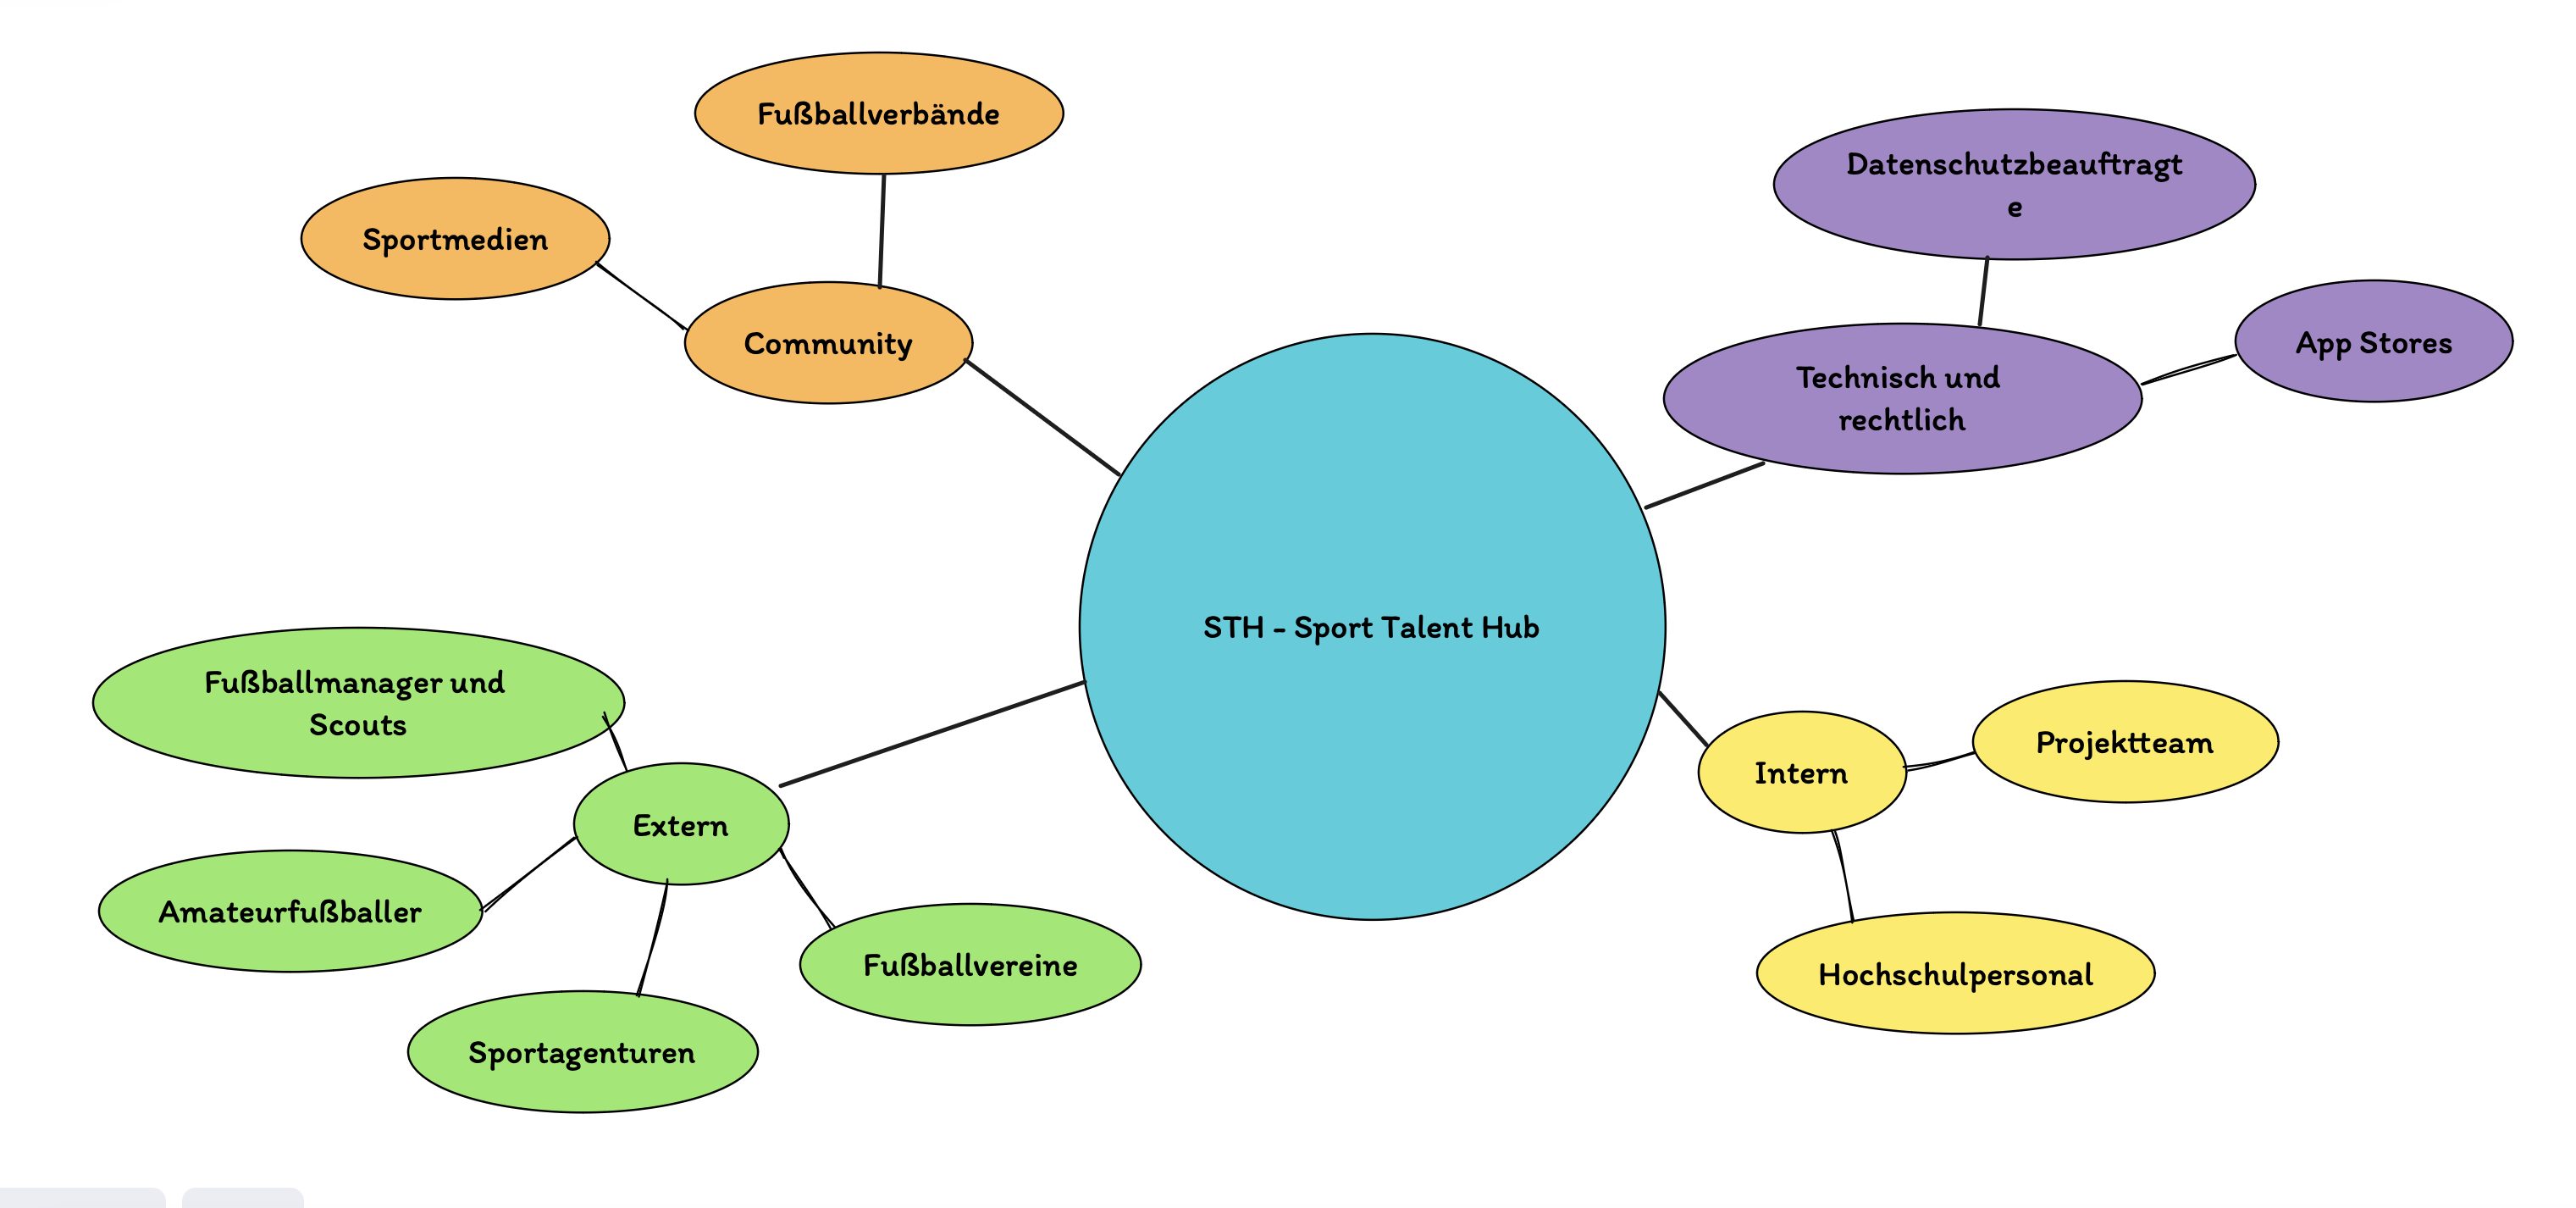
\includegraphics[width=\textwidth]{assets/figures/Stakeholderanalyse.png}
    \begin{flushleft}
		Quelle: Quelle Stakeholderanalyse
	\end{flushleft}
\end{figure}

